\chapter{Technical Approach}
\label{ch:approach}

%-------------------------------------------------------

\section{Pipeline overview}

Figure~\ref{fig:pipeline} shows the complete pipeline. A photo first goes through \emph{localisation}, which finds the outline of each card as a quadrilateral, and \emph{rectification}, which warps each card to a canonical front view of $500\times700$ pixels (the 5:7 shape of a 63\,mm\,$\times$\,88\,mm card). The rectified card is then passed to a \emph{retrieval method}, which ranks all reference cards. All retrieval methods share one interface, so that every method receives exactly the same rectified input and is evaluated by the same code. Language recognition and the condition estimate run after identification, in the application.

\begin{figure}[htbp]
\centering
\begin{tikzpicture}[
    node distance=6mm and 5mm,
    box/.style={draw, rounded corners=2pt, align=center, font=\small, minimum height=10mm, text width=27mm, fill=blue!4},
    opt/.style={box, fill=gray!8, dashed},
    arr/.style={-{Stealth[length=2mm]}, thick}]
  \node[box] (photo) {Photo\\(one or more cards)};
  \node[box, right=of photo] (loc) {Localisation\\Canny, contours,\\hull, 4 corners};
  \node[box, right=of loc] (rect) {Rectification\\homography to\\$500\times700$};
  \node[box, right=of rect] (ret) {Retrieval\\rank all \res{db-cards}\\reference cards};
  \node[box, below=10mm of ret, text width=60mm] (methods) {\textbf{Methods (one interface):} pixel, ORB / SIFT + RANSAC, ResNet-50, CLIP, hybrid (embedding top-$k$ $\to$ SIFT + RANSAC); variants +rot, @art};
  \node[opt, below=10mm of loc] (lang) {Printed language\\(OCR + rules)};
  \node[opt, below=10mm of photo] (cond) {Condition estimate\\(photo vs.\ scan)};
  \draw[arr] (photo) -- (loc);
  \draw[arr] (loc) -- (rect);
  \draw[arr] (rect) -- (ret);
  \draw[arr, dashed] (methods) -- (ret);
  \draw[arr, dashed] (rect.south) |- ++(0,-4mm) -| (lang.north);
  \draw[arr, dashed] (lang) -- (cond);
\end{tikzpicture}
\caption[Pipeline overview]{Pipeline overview. Solid arrows: the identification pipeline that is evaluated in this report. Dashed boxes: extensions used by the application (Section~\ref{sec:extensions}).}
\label{fig:pipeline}
\end{figure}

\section{Card localisation}
\label{sec:localisation}

The detector (\texttt{cardrec/rectify.py}) is fully classical and has no learned parameters. Its design goal is to find the \emph{outer} outline of the card, not an inner frame such as the artwork box, under perspective, blur and glare.

\begin{enumerate}
  \item \textbf{Edge maps.} The photo is downscaled so that its longest side is at most 800 pixels and smoothed with a $5\times5$ Gaussian filter. Two channels are used: grey level and the HSV saturation, because a silver card border can have the same brightness as the table but a different colourfulness. On each channel the Canny detector \citep{canny1986edge} is run with three threshold pairs (fixed $50/150$, relative to the median grey level $0.5m/1.0m$, and low $10/40$ for blurry photos), and each edge map is dilated with a $3\times3$ kernel once (keeps the thin gap between touching cards) and twice (closes gaps in blurry edges). All twelve edge maps are used.
  \item \textbf{Candidate quadrilaterals.} Contours are extracted from every edge map \citep{suzuki1985contours}. For each contour, its convex hull is simplified with the Douglas--Peucker algorithm \citep{douglas1973peucker}, with a tolerance that grows from 2\% to 8\% of the perimeter until four corners remain. Using the hull instead of the raw contour makes the step robust to rounded card corners and to edges broken by glare.
  \item \textbf{Checks.} A quadrilateral is kept only if (i) its area is at least 3\% of the image, (ii) it does not touch the image border, (iii) its aspect ratio (long side / short side) is between 1.15 and 1.95 (a real card is $88/63\approx1.40$; perspective changes it), (iv) the contour fills at least 85\% of the quadrilateral, and (v) its four sides lie on real edges: of 60 points sampled along each side, at least 60\% must be edge pixels (``edge support''). The last check rejects large shapes stretched around background noise.
  \item \textbf{Selection.} Candidates are sorted by $\text{score} = \text{area}\times\text{support}^2$, so that a quadrilateral that also covers some background (lower support) loses to the true card outline. A candidate is dropped if its centre lies inside an already accepted card (inner frames) or if it overlaps one with intersection-over-union (IoU) above 0.5 (duplicates from different edge maps). Up to ten cards are returned.
\end{enumerate}

If no candidate passes, the single-card pipeline falls back to resizing the whole photo to $500\times700$. The thresholds were tuned only on separate development query sets, never on the test queries described in Chapter~\ref{ch:data}.

\section{Rectification}
\label{sec:rectification}

The four corners are ordered by their angle around the centroid and the list starts at the corner with the smallest $x+y$, which becomes the top-left corner of the output. If the top side is longer than the left side, the card is lying sideways and the order is rotated by one position. The perspective transform $H$ that maps the four corners $\mathbf{p}_i$ to the corners of the $500\times700$ rectangle $\mathbf{q}_i$ is computed exactly from the four correspondences,
\begin{equation}
  \lambda_i \begin{pmatrix} \mathbf{q}_i \\ 1 \end{pmatrix} = H \begin{pmatrix} \mathbf{p}_i \\ 1 \end{pmatrix}, \qquad i = 1,\dots,4,
  \label{eq:homography}
\end{equation}
and the photo is warped with $H$. This step cannot tell the top of the card from the bottom: a card rotated by $180^\circ$ produces a valid but upside-down rectification. With the corner ordering above, cards rotated by about $-45^\circ$ to $+135^\circ$ come out upright and other rotations come out upside down. Keypoint methods are rotation invariant and do not care; for the embedding methods, the ``+rot'' variant (Section~\ref{sec:variants}) addresses it.

\section{Retrieval interface}

Every method implements two operations: \texttt{build\_index(reference images, ids)}, run once, and \texttt{query(rectified card)}, which returns the \emph{complete} ranking of the database as (id, score) pairs. Reference scans are resized to the same $500\times700$ canonical size as the queries. Indexes are cached on disk, so the expensive index of the keypoint methods is computed only once.

\paragraph{Keypoint matching with RANSAC.} For SIFT \citep{lowe2004sift} and ORB \citep{rublee2011orb}, up to 800 keypoints are detected on the grey-level card. Each query descriptor is matched to its two nearest neighbours in a reference card by brute force (L2 distance for SIFT, Hamming distance for ORB), and a match is kept if it passes the ratio test with ratio 0.75. If at least four matches remain, a homography is estimated with RANSAC \citep{fischler1981ransac} using a reprojection threshold of 5 pixels, and the \emph{number of inliers} is the similarity score. The query is compared with every reference card.

\paragraph{Global embeddings.} An embedding method maps an image to a vector $\mathbf{f}$, normalised to unit length. The similarity between the query $\mathbf{f}_q$ and a reference $\mathbf{f}_r$ is the cosine similarity $s(q,r) = \mathbf{f}_q^\top\mathbf{f}_r$, computed for all references with one matrix product.

\section{Hybrid re-ranking}
\label{sec:hybrid}

The hybrid combines a fast embedding with precise geometric verification, in the spirit of spatial re-ranking \citep{philbin2007spatial}. Let $S_k$ be the $k$ references with the highest embedding similarity to the query. Only these $k$ cards are verified with SIFT + RANSAC, and they are re-ordered by
\begin{equation}
  \text{rank within } S_k \text{ by } \big(\, \text{inliers}(q,r) \downarrow,\;\; s(q,r) \downarrow \,\big),
  \label{eq:hybrid}
\end{equation}
that is, by the number of RANSAC inliers, with ties broken by the embedding similarity. The cards outside the shortlist keep their embedding order after the $k$ re-ranked cards, so the output is still a full ranking. The default shortlist size is $k=20$, so SIFT matching is done against 20 cards instead of \res{db-cards}. If the correct card is not in the shortlist, the hybrid cannot recover it; this is why the shortlist size is a parameter of the experiments.

\section{Variants}
\label{sec:variants}

\begin{itemize}
  \item \textbf{+rot} (embedding and hybrid methods only). The query is embedded twice, as rectified and rotated by $180^\circ$, and each reference keeps the higher of the two similarities. This removes the up/down ambiguity of the rectification at the cost of a second forward pass.
  \item \textbf{@art}. Both the references and the query are cropped to a fixed artwork window (rows 70--340, columns 35--465 of the $500\times700$ card) before indexing and querying. The window contains no text, so it is the same in every language. On full-art cards it is simply the upper-middle part of the illustration.
\end{itemize}

\section{Extensions used by the application}
\label{sec:extensions}

\paragraph{Printed language.} Identification and language are treated as separate problems. The card is identified from its image (for non-English cards, preferably with an @art method), and the printed language is classified separately (\texttt{cardrec/language.py}). The rectified card is re-warped at $750\times1050$ pixels, because the small text is unreadable at $500\times700$, and read by EasyOCR twice, once with a Japanese+English reader and once with a Spanish+English reader. Fixed rules then decide: (1) if kana characters (hiragana and katakana) make up at least 30\% of the letters read by the Japanese reader, the card is Japanese (kanji are not counted, because the reader invents kanji on blurry Latin text); (2) otherwise, the language code printed next to the set code at the bottom left (for example ``PRE EN'') is read in an enlarged crop; (3) otherwise, typical English and Spanish words and Spanish accented characters are counted, and the larger count wins; with no evidence the answer is ``unknown''.

\paragraph{Visual condition estimate.} Once a card is identified, its official scan is a picture of the undamaged card. The condition module (\texttt{cardrec/condition.py}) re-detects the outline precisely, warps the photo to $750\times1050$ pixels (about 12 pixels per millimetre), aligns the scan to the photo with SIFT + RANSAC and matches the colours. It then measures centering from the border widths, three sub-scores (whitening, fill, fray) for each of the four corners and four edges, and surface defects as remaining differences between photo and scan. These are combined into a 0--1000 score with hand-set weights. The result is explicitly labelled as an \emph{estimate}, not an official grade.

\paragraph{Application.} A local web application called CardDex (Flask back end, single-page front end, SQLite collection) puts the pipeline into practice (Figure~\ref{fig:app-screens}). The user uploads a photo and chooses one of eight retrieval methods (SIFT by default); a one-sentence description of each method, with its typical speed, is shown next to the selector, so that a user without a computer-vision background can choose, for example, the fast CLIP hybrid for everyday use or the artwork-only hybrid for non-English cards. The application detects and rectifies the card, ranks the reference cards with the selected method and shows the top-5 candidates with their scores, so that a wrong first guess can be corrected by clicking another candidate. For inlier-based methods it marks a result as a likely match when the best card has at least 15 inliers and at least 1.4 times the inliers of the second card. It then shows tags derived from the card metadata (set, number, name, category, stage, type, rarity, regulation mark, illustrator), classifies the printed language, optionally estimates the condition from a front and a back photo, and saves the card to a personal collection with its quantity, language and a market price (TCGdex first, Pok\'emon TCG API as fallback, cached for 24 hours). The collection panel can be filtered by every tag. Besides the \res{db-cards} English reference cards, the application's database contains the \res{db-ja-cards} cards of the Japanese set \emph{Battle Partners} (official scans from TCGdex), so that Japanese copies can be identified as Japanese cards and not only as their English counterparts. \res{db-ja-linked} of them were linked to the English card with the same artwork using the rule of the cross-language test set (Section~\ref{sec:langdata}), and all links were checked by eye. When the best match is a Japanese card, the application pre-selects Japanese as the language of the user's copy, and its price is taken from TCGdex's Japanese catalogue (Cardmarket, in EUR). These Japanese cards are used only by the application, not in the benchmark experiments of this report. The application is started with \texttt{run\_app.bat} or \texttt{python -m cardrec.app.server}; it runs locally and needs internet access only for prices.

\begin{figure}[htbp]
\centering
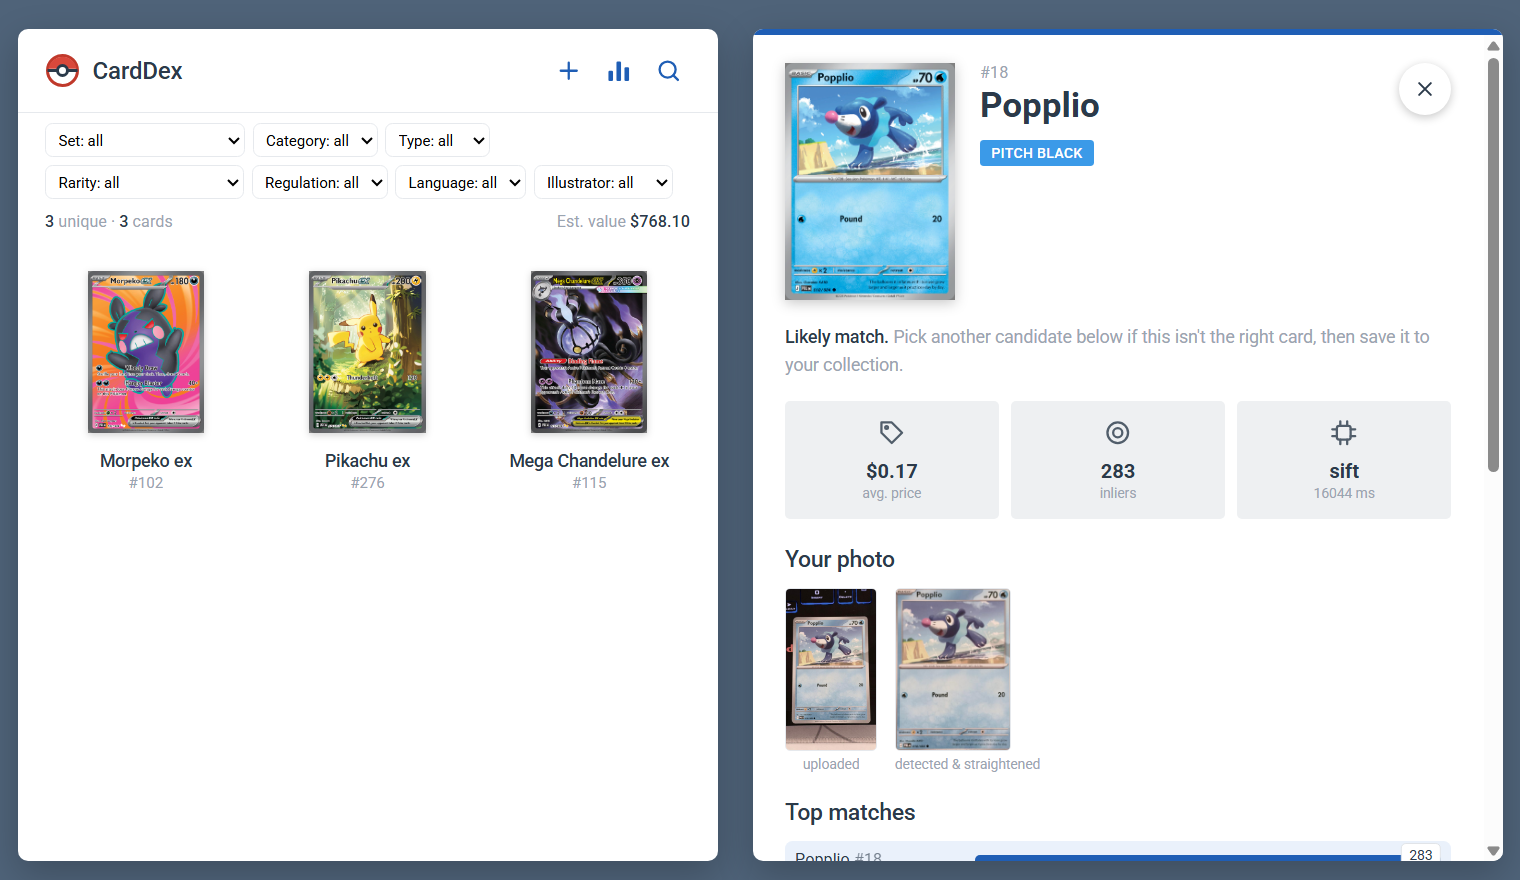
\includegraphics[width=\textwidth]{figures/app_analysis.png}\\[4pt]
\begin{subfigure}{0.49\textwidth}\centering
  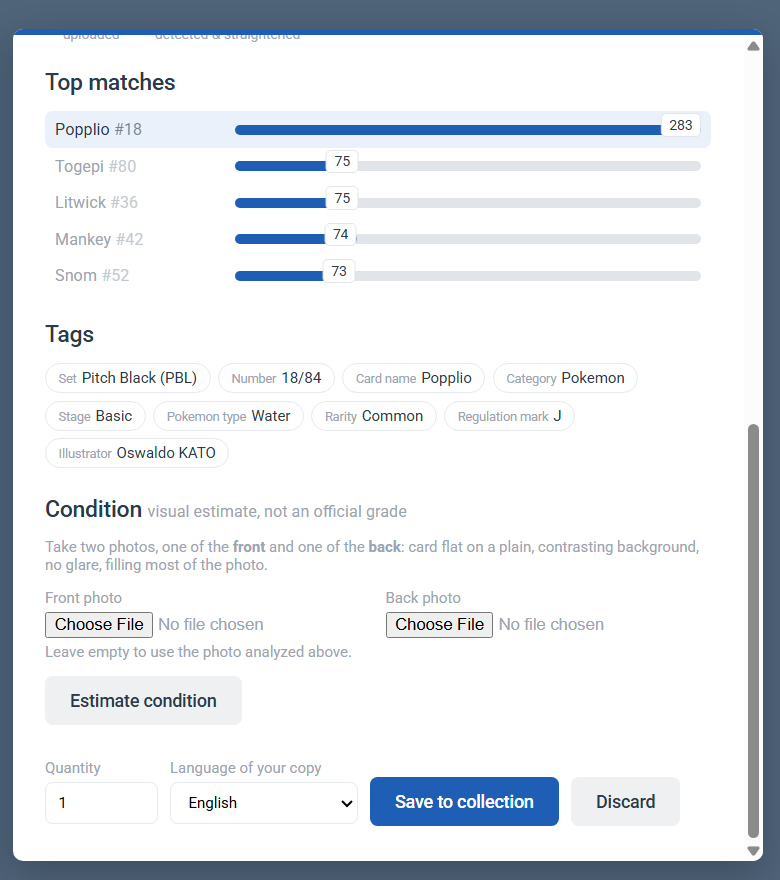
\includegraphics[width=\textwidth]{figures/app_matches_tags.png}
  \caption{Top-5 matches, tags and saving.}\label{fig:app-matches}
\end{subfigure}\hfill
\begin{subfigure}{0.49\textwidth}\centering
  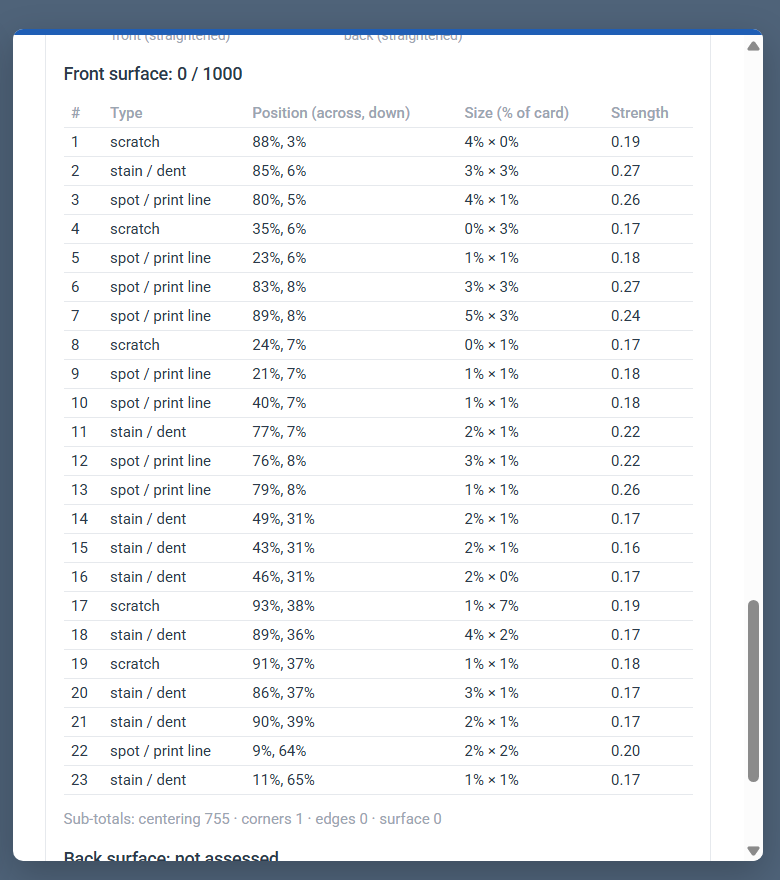
\includegraphics[width=\textwidth]{figures/app_surface.png}
  \caption{Condition report: surface table.}\label{fig:app-surface}
\end{subfigure}
\caption[The CardDex application]{The CardDex application (screenshots by the author on 1 November 2026, browser frame removed; the collection shown is the one at that date). Top: collection with tag filters (left) and the analysis of an uploaded phone photo (right): best match, average price, number of RANSAC inliers, method and time, and the uploaded and straightened photo. (a) The ranked candidates, the tags taken from the database and the save form. (b) Part of the condition report of the same card.}
\label{fig:app-screens}
\end{figure}
